\chapter{Hipótesis}

La hipótesis que se maneja en este estudio se basa en el estudio de modelos sólidos que postulan que la materia oscura está compuesta de partículas elementales, las cuales no han sido observadas hasta este momento, sin embargo podrían ser producidas en el laboratorio. De ser esto cierto se requiere de un nuevo marco teórico, es decir una teoría que más allá del modelo estándar sustente dicha hipótesis.
Afortunadamente ya existen varios modelos propuestos que predicen dicha
producción, uno de los modelos más populares es el del llamado sector oscuro, o dark sector, el cual lo explica desde el rompimiento de una simetría que da lugar a la producción del llamado fotón oscuro (dark photon); dicha partícula sería la partícula portadora entre el sector oscuro y el del modelo estándar, es decir un bosón, y la interacción entre estos dos sectores se daría por medio de lo que se conoce como el parámetro cinético de mezcla (kinetic mixing parameter), usualmente abreviado como [], el cual mide la interacción entre los dos sectores.

Una de las características de esta nueva partícula, y que la diferencia del fotón del modelo estándar, es que sería masiva y que su tiempo de vida podría ser significativo. En esta teoría esta nueva partícula tendría dos parámetros libres (masa y tiempo de vida), además de que su detección se dará de forma indirecta, es decir por el decaimiento a partículas del modelo estándar. Uno de los canales más prometedores es en el que el fotón oscuro decae a muones que si son partículas que pueden ser identificadas y reconstruidas con gran eficacia usando el detector CMS como se comentó en la sección 1.3, por lo que la probabilidad de detección es mayor que con otros modos de decaimientos.

\begin{figure}
    \centering
    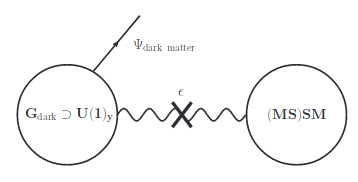
\includegraphics[width=0.7\textwidth]{HIPOTESIS/sketch_darksector.png}
    \caption{. Ilustración esquemática de la conexión entre el sector oscuro y el modelo estándar, los cuales están conectados mediante un término de mezcla dinámica.}
    \label{fig:sketch_darksector}
\end{figure}

Adicionalmente en varios de estos modelos el bosón de Higgs puede servir como
portal del sector oscuro [], es decir, existe la probabilidad de que uno de los decaimientos del bosón de Higgs sea a partículas como el fotón oscuro; esto es válido para el bosón de Higgs del modelo estándar, recientemente observado y cuya masa es de 125 GeV, pero también podría ser válido en teorías que predicen más de un bosón de Higgs, incluso con aquellos que postulan la existencia de partículas
supersimétricas.














